\documentclass[10pt,aspectratio=169]{beamer}
\usepackage[utf8]{inputenc}
\usepackage{listings}
\usepackage{hyperref}
\usepackage{xcolor}
\usepackage{ragged2e}
\usepackage{graphicx}
\usepackage{tikz}
\usetikzlibrary{positioning,calc,decorations.pathreplacing}

\usetheme{Dresden}
%\usetheme{Bergen}

\title{Programming Techniques 2026--2027}
\author{Hannu Parviainen}
\institute{Universidad de la Laguna}
\date{\today}

% Single spaces after full stops, so that e.g. \texttt{a .dot. b} has even spacing
\frenchspacing

\lstset{
  language=fortran,
  basicstyle=\ttfamily\scriptsize,
  columns=fullflexible,
  keepspaces=true,
  backgroundcolor=\color{white},
  keywordstyle=\color{blue},
  commentstyle=\color{gray},
  stringstyle=\color{red},
  showstringspaces=false,
  breaklines=true,
  frame=lines
}

\subtitle{Lecture 7: Formatted and File I/O, and Makefiles}

\begin{document}

\begin{frame}
  \titlepage
\end{frame}

\section{Recap}

\begin{frame}[fragile]
  \frametitle{Recap: basic I/O}
  \begin{columns}[T]
    \begin{column}{0.45\textwidth}
      \begin{itemize}
        \item In \texttt{read(unit, fmt)} and \texttt{write(unit, fmt)}, the unit comes first and the format second.
        \item A \texttt{*} unit is the terminal. A \texttt{*} format is list-directed: the compiler chooses the layout.
        \item \texttt{iostat=ios} is 0 on success, negative at the end of the input, and positive on an error. \texttt{iomsg=msg} gives the message.
        \item An internal read reads from a string: \texttt{read(line, *) x}.
        \item Redirection: \mbox{\texttt{./a.out < in.txt > out.txt}}.
      \end{itemize}
    \end{column}

    \begin{column}{0.55\textwidth}
      \vspace*{2mm}
      \centering
      \footnotesize
      \begin{tabular}{lll}
        \textbf{Statement} & \textbf{Unit} & \textbf{Format} \\
        \hline
        \texttt{print *, x}           & std.\ output & list-directed \\
        \texttt{write(*, *) x}        & std.\ output & list-directed \\
        \texttt{read *, x}            & std.\ input  & list-directed \\
        \texttt{read(*, *) x}         & std.\ input  & list-directed \\
        \texttt{read(line, *) x}      & a string     & list-directed \\
        \hline
        \texttt{write(u, '(f8.3)') x} & a file       & explicit \\
      \end{tabular}

      \vspace*{4mm}
      \normalsize
      \raggedright
      Today: explicit formats, files, command-line arguments, and building programs with \texttt{make}.
    \end{column}
  \end{columns}
\end{frame}


\section{Formatted I/O}

\begin{frame}
  \centering
  \Huge \textbf{Formatted Input and Output}
\end{frame}


\begin{frame}[fragile]
  \frametitle{Format specifications}
  \begin{columns}[T]
    \begin{column}{0.45\textwidth}
      \begin{itemize}
        \item A format is a string in parentheses that replaces the \texttt{*} format.
        \item It has one \emph{edit descriptor} for each item. Quoted text inside it is written as it is.
        \item A format can be stored in a named constant and reused.
        \item Formatted output does not start with a space.
        \item Old code uses labelled \texttt{format} statements: \texttt{write(*, 100) x} with \texttt{100 format(f8.3)}.
      \end{itemize}
    \end{column}

    \begin{column}{0.55\textwidth}
      \begin{lstlisting}
program formats
  implicit none
  character(len=*), parameter :: fmt = '(a, f8.3, a)'
  real :: period = 365.25636

  print *, 'Period:', period, 'days'
  print '(a, f8.3, a)', 'Period:', period, ' days'
  write(*, fmt) 'Period:', period, ' days'
  write(*, '("Period: ", f0.1, " days")') period
end program formats
      \end{lstlisting}
      \begin{lstlisting}[language=bash]
$ gfortran formats.f90 && ./a.out
 Period:   365.256348     days
Period: 365.256 days
Period: 365.256 days
Period: 365.3 days
      \end{lstlisting}
    \end{column}
  \end{columns}
\end{frame}


\begin{frame}[fragile]
  \frametitle{Edit descriptors}
  \begin{columns}[T]
    \begin{column}{0.45\textwidth}
      \small
      \begin{tabular}{@{}ll@{}}
        \texttt{Iw}     & integer, field width \texttt{w} \\
        \texttt{Iw.m}   & integer, at least \texttt{m} digits \\
        \texttt{Fw.d}   & real, \texttt{d} decimals \\
        \texttt{ESw.d}  & real, scientific notation \\
        \texttt{Ew.d}   & real, exponential notation \\
        \texttt{Aw}     & string (\texttt{A}: its own length) \\
        \texttt{Lw}     & logical, \texttt{T} or \texttt{F} \\
        \texttt{G0}     & any type, minimal width \\
        \texttt{nX}     & skip \texttt{n} positions \\
        \texttt{/}      & start a new line \\
        \texttt{"text"} & the text itself \\
      \end{tabular}

      \vspace*{2mm}
      \normalsize
      \begin{itemize}
        \item The width \texttt{w} includes the sign and the decimal point.
        \item Values are right-aligned in their field.
      \end{itemize}
    \end{column}

    \begin{column}{0.55\textwidth}
      \begin{lstlisting}
program descriptors
  implicit none
  integer :: n = 42
  real :: d = 456.789, m = 1.989e30
  print '(i5, "|", i5.4, "|", i0)', n, n, n
  print '(f8.2, "|", es10.3, "|", e10.3)', d, d, d
  print '(g0, "|", g0, "|", g0)', n, d, m
  print '(a, "|", a6, "|", l2)', 'Sun', 'Sun', .true.
  print '(i3, 4x, i3, /, i3)', 1, 2, 3
end program descriptors
      \end{lstlisting}
      \begin{lstlisting}[language=bash]
$ gfortran descriptors.f90 && ./a.out
   42| 0042|42
  456.79| 4.568E+02| 0.457E+03
42|456.789001|0.198900001E+31
Sun|   Sun| T
  1      2
  3
      \end{lstlisting}
    \end{column}
  \end{columns}
\end{frame}


\begin{frame}[fragile]
  \frametitle{Field widths, repeats, and groups}
  \begin{columns}[T]
    \begin{column}{0.45\textwidth}
      \begin{itemize}
        \item Width 0 is the minimum width: \texttt{i0}, \texttt{f0.2}. Good in text, but columns will not line up, and gfortran drops the zero before the decimal point.
        \item A value too wide for its field gives \texttt{***}.
        \item Repeat counts: \texttt{3f8.2}. Groups: \texttt{3(f5.2, ";")}.
        \item \texttt{*(...)} repeats a group as often as needed: one format for an array of any size.
        \item When the format runs out, the output goes on to a new line and reuses the last group.
      \end{itemize}
    \end{column}

    \begin{column}{0.55\textwidth}
      \begin{lstlisting}
program widths
  implicit none
  real :: r(5) = [0.5, -2.5, 3.25, 10.0, 12345.6]
  print '(i3, "|", i0, "|", f6.1)', 12345, 12345, r(5)
  print '(3f8.2)', r(1:3)
  print '(3(f5.2, ";"))', r(1:3)
  print '(a, *(1x, f0.2))', 'r =', r
  print '(2f8.2)', r
end program widths
      \end{lstlisting}
      \begin{lstlisting}[language=bash]
$ gfortran widths.f90 && ./a.out
***|12345|******
    0.50   -2.50    3.25
 0.50;-2.50; 3.25;
r = .50 -2.50 3.25 10.00 12345.60
    0.50   -2.50
    3.25   10.00
12345.60
      \end{lstlisting}
    \end{column}
  \end{columns}
\end{frame}


\begin{frame}[fragile]
  \frametitle{Internal write and non-advancing output}
  \begin{columns}[T]
    \begin{column}{0.45\textwidth}
      \begin{itemize}
        \item An \emph{internal write} writes into a string, the reverse of an internal read.
        \item Use it to build file names: \texttt{'(a, i4.4, a)'} gives \texttt{snap\_0010.dat}.
        \item The rest of the string is filled with spaces, so use \texttt{trim}.
        \item \texttt{advance='no'} keeps the line open. It needs an explicit format.
      \end{itemize}
      \begin{lstlisting}[language=bash]
$ gfortran internal_write.f90 && ./a.out
snap_0010.dat
snap_0020.dat
snap_0030.dat
Steps: 1 2 3 4 5 finished
      \end{lstlisting}
    \end{column}

    \begin{column}{0.55\textwidth}
      \begin{lstlisting}
program internal_write
  implicit none
  character(len=100) :: fname
  integer :: i
  do i = 1, 3
    write(fname, '(a, i4.4, a)') 'snap_', 10*i, '.dat'
    print '(a)', trim(fname)
  end do
  write(*, '(a)', advance='no') 'Steps:'
  do i = 1, 5
    write(*, '(1x, i0)', advance='no') i
  end do
  write(*, '(a)') ' finished'
end program internal_write
      \end{lstlisting}
    \end{column}
  \end{columns}
\end{frame}


\section{Files}

\begin{frame}
  \centering
  \Huge \textbf{Files}
\end{frame}


\begin{frame}[fragile]
  \frametitle{Opening and closing files}
  \begin{columns}[T]
    \begin{column}{0.45\textwidth}
      \begin{itemize}
        \item \texttt{open} connects a file to a unit, and \texttt{close} disconnects it.
        \item \texttt{newunit=u}: the compiler picks a free unit. Avoid fixed numbers like 10.
        \item \texttt{status='old'}, \texttt{'new'}, or \texttt{'replace'}. \texttt{action='read'}, \texttt{'write'}, or \texttt{'readwrite'}. \texttt{position='append'} writes at the end.
        \item Check \texttt{iostat}: missing files and wrong paths are the most common I/O errors.
      \end{itemize}
    \end{column}

    \begin{column}{0.55\textwidth}
      \begin{lstlisting}[aboveskip=0pt, belowskip=0pt]
program write_table
  implicit none
  real, parameter :: a(3) = [0.39, 0.72, 1.00]
  character(len=200) :: msg
  integer :: u, ios, i
  open(newunit=u, file='orbits.txt', status='replace', &
       action='write', iostat=ios, iomsg=msg)
  if (ios /= 0) error stop trim(msg)
  write(u, '(a)') '# a [AU]  P [yr]'
  do i = 1, size(a)
    write(u, '(f8.2, f8.3)') a(i), a(i)**1.5
  end do
  close(u)
end program write_table
      \end{lstlisting}
      \begin{lstlisting}[language=bash, aboveskip=2pt]
$ gfortran write_table.f90 && ./a.out && cat orbits.txt
# a [AU]  P [yr]
    0.39   0.244
    0.72   0.611
    1.00   1.000
      \end{lstlisting}
    \end{column}
  \end{columns}
\end{frame}


\begin{frame}[fragile]
  \frametitle{Reading a file of unknown length}
  \begin{columns}[T]
    \begin{column}{0.45\textwidth}
      \begin{itemize}
        \item A file is read like the keyboard, with the unit in place of \texttt{*}.
        \item \texttt{iostat\_end} (in \texttt{iso\_fortran\_env}) is the \texttt{iostat} value at the end of a file.
        \item \texttt{read(u, *)} with no variables skips a line, and \texttt{rewind(u)} goes back to the start.
        \item Two passes allocate the arrays once, instead of growing them for each value (Lecture 5).
      \end{itemize}
      \begin{lstlisting}[language=bash]
$ gfortran read_table.f90 && ./a.out
3 planets, max P 1.00
      \end{lstlisting}
    \end{column}

    \begin{column}{0.55\textwidth}
      \begin{lstlisting}[aboveskip=0pt, belowskip=0pt]
program read_table
  use iso_fortran_env, only: iostat_end
  implicit none
  real, allocatable :: a(:), p(:)
  integer :: u, ios, n, i
  open(newunit=u, file='orbits.txt', action='read')
  n = -1                     ! do not count the header
  do                         ! 1st pass: count lines
    read(u, *, iostat=ios)
    if (ios == iostat_end) exit
    n = n + 1
  end do
  allocate(a(n), p(n))
  rewind(u)                  ! 2nd pass: read values
  read(u, *)                 ! skip the header
  do i = 1, n
    read(u, *) a(i), p(i)
  end do
  close(u)
  print '(i0, " planets, max P ", f0.2)', n, maxval(p)
end program read_table
      \end{lstlisting}
    \end{column}
  \end{columns}
\end{frame}


\begin{frame}[fragile]
  \frametitle{Checking files and reporting errors}
  \begin{columns}[T]
    \begin{column}{0.45\textwidth}
      \begin{itemize}
        \item \texttt{inquire(file=name, exist=found)} checks whether a file exists.
        \item \texttt{iso\_fortran\_env} names the standard units: \texttt{input\_unit}, \texttt{output\_unit}, and \texttt{error\_unit}.
        \item Messages written to \texttt{error\_unit} stay on the terminal when the output is redirected.
        \item \texttt{flush(u)} writes buffered output to the file now, so you can follow a long run.
      \end{itemize}
    \end{column}

    \begin{column}{0.55\textwidth}
      \begin{lstlisting}
program check_file
  use iso_fortran_env, only: error_unit
  implicit none
  logical :: found
  inquire(file='input.dat', exist=found)
  if (.not. found) then
    write(error_unit, '(a)') 'Error: input.dat not found'
    stop 1
  end if
  print '(a)', 'Found input.dat'
end program check_file
      \end{lstlisting}
      \begin{lstlisting}[language=bash]
$ gfortran check_file.f90
$ ./a.out > out.txt
Error: input.dat not found
STOP 1
      \end{lstlisting}
    \end{column}
  \end{columns}
\end{frame}


\section{Arguments}

\begin{frame}[fragile]
  \frametitle{Command-line arguments}
  \begin{columns}[T]
    \begin{column}{0.45\textwidth}
      \begin{itemize}
        \item \texttt{command\_argument\_count()} gives the number of arguments.
        \item \texttt{call get\_command\_argument(i, arg)} copies argument \texttt{i} into \texttt{arg} (0 is the program name).
        \item Arguments are text: convert numbers with an internal read.
      \end{itemize}
      \begin{lstlisting}[language=bash]
$ gfortran -o args args.f90
$ ./args
Usage: ./args <input file> <steps>
STOP 1
$ ./args input.dat 1000
Reading input.dat, running 1000 steps
      \end{lstlisting}
    \end{column}

    \begin{column}{0.55\textwidth}
      \begin{lstlisting}
program args
  implicit none
  character(len=256) :: fname, arg
  integer :: nsteps
  if (command_argument_count() /= 2) then
    print '(a)', 'Usage: ./args <input file> <steps>'
    stop 1
  end if
  call get_command_argument(1, fname)
  call get_command_argument(2, arg)
  read(arg, *) nsteps
  print '(3a, i0, a)', 'Reading ', trim(fname), &
                       ', running ', nsteps, ' steps'
end program args
      \end{lstlisting}
    \end{column}
  \end{columns}
\end{frame}


\section{Makefiles}

\begin{frame}
  \centering
  \Huge \textbf{Makefiles}
\end{frame}


\begin{frame}[fragile]
  \frametitle{Why build tools?}
  \begin{columns}[T]
    \begin{column}{0.5\textwidth}
      \begin{itemize}
        \item A real program has many modules, and modules use other modules that use other modules\ldots
        \item A module must be compiled before any code that uses it, because the compiler reads its \texttt{.mod} file.
        \item When a module changes, everything that uses it must be recompiled, and the program linked again.
        \item You do not want to do this by hand. A build tool does it for you, and recompiles only what has changed.
      \end{itemize}
    \end{column}

    \begin{column}{0.5\textwidth}
      \centering
      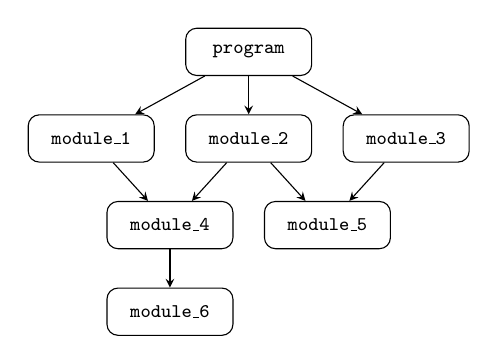
\begin{tikzpicture}[
          box/.style={draw, rounded corners, minimum width=16mm, minimum height=6mm, font=\scriptsize\ttfamily},
          uses/.style={->, >=stealth}]
        \node[box] (p) at (0, 0) {program};
        \node[box] (m1) at (-2, -1.1) {module\_1};
        \node[box] (m2) at ( 0, -1.1) {module\_2};
        \node[box] (m3) at ( 2, -1.1) {module\_3};
        \node[box] (m4) at (-1, -2.2) {module\_4};
        \node[box] (m5) at ( 1, -2.2) {module\_5};
        \node[box] (m6) at (-1, -3.3) {module\_6};
        \draw[uses] (p) -- (m1);
        \draw[uses] (p) -- (m2);
        \draw[uses] (p) -- (m3);
        \draw[uses] (m1) -- (m4);
        \draw[uses] (m2) -- (m4);
        \draw[uses] (m2) -- (m5);
        \draw[uses] (m3) -- (m5);
        \draw[uses] (m4) -- (m6);
      \end{tikzpicture}

      \vspace*{1mm}
      {\scriptsize An arrow means ``uses''. If \texttt{module\_6} changes, \texttt{module\_4}, \texttt{module\_1}, \texttt{module\_2}, and the program must all be recompiled.}
    \end{column}
  \end{columns}
\end{frame}


\begin{frame}[fragile]
  \frametitle{Make and makefile rules}
  \begin{columns}[T]
    \begin{column}{0.5\textwidth}
      \begin{itemize}
        \item \texttt{make} runs the commands needed to build a target, using the rules in a file called \texttt{makefile}.
        \item A rule has a target, its dependencies, and the commands that make the target:\\[1mm]
          \texttt{target: dep\_1 dep\_2}\\
          \texttt{\phantom{xxxx}command}
        \item Commands must start with a \textbf{TAB}, not spaces. Text copied from a PDF has spaces!
        \item A target is rebuilt only if it is missing or older than one of its dependencies.
        \item \texttt{make} builds the first target, and \texttt{make clean} the target \texttt{clean}.
      \end{itemize}
    \end{column}

    \begin{column}{0.5\textwidth}
      \begin{lstlisting}[language={[gnu]make}, tabsize=4]
all: e1

e1: m1.o e1.o
	gfortran -o e1 m1.o e1.o

m1.o: m1.f90
	gfortran -c m1.f90

# e1.f90 uses the module m1
e1.o: e1.f90 m1.o
	gfortran -c e1.f90

clean:
	rm -f *.o *.mod e1
      \end{lstlisting}
    \end{column}
  \end{columns}
\end{frame}


\begin{frame}[fragile]
  \frametitle{Running make}
  \begin{columns}[T]
    \begin{column}{0.45\textwidth}
      \begin{itemize}
        \item \texttt{make} prints each command before it runs it.
        \item A second \texttt{make} does nothing, because every target is newer than its dependencies.
        \item \texttt{touch} updates the modification time of a file, as if it had been edited. After \texttt{touch m1.f90}, \texttt{make} recompiles \texttt{m1.o}, then \texttt{e1.o}, which depends on it, and links the program again.
        \item The example makefiles are in \texttt{examples/ex08\_makefiles}.
      \end{itemize}
    \end{column}

    \begin{column}{0.55\textwidth}
      \begin{lstlisting}[language=bash, deletekeywords={done, for}]
$ make
gfortran -c m1.f90
gfortran -c e1.f90
gfortran -o e1 m1.o e1.o
$ make
make: Nothing to be done for 'all'.
$ touch m1.f90
$ make
gfortran -c m1.f90
gfortran -c e1.f90
gfortran -o e1 m1.o e1.o
$ make clean
rm -f *.o *.mod e1
      \end{lstlisting}
    \end{column}
  \end{columns}
\end{frame}


\begin{frame}[fragile]
  \frametitle{Variables and automatic variables}
  \begin{columns}[T]
    \begin{column}{0.5\textwidth}
      \begin{itemize}
        \item \texttt{NAME = value} defines a variable, and \texttt{\$(NAME)} is replaced by its value.
        \item By convention, \texttt{FC} is the Fortran compiler and \texttt{FCFLAGS} holds the compiler options.
        \item Variables can be overridden on the command line: \texttt{make FCFLAGS="-g -O0"}.
        \item Automatic variables, set for each rule:
          \begin{itemize}
            \item \texttt{\$@}: the target,
            \item \texttt{\$<}: the first dependency,
            \item \texttt{\$\^{}}: all the dependencies.
          \end{itemize}
      \end{itemize}
    \end{column}

    \begin{column}{0.5\textwidth}
      \begin{lstlisting}[language={[gnu]make}, tabsize=4]
FC = gfortran
FCFLAGS = -Wall -O2
OBJECTS = m1.o e1.o

e1: $(OBJECTS)
	$(FC) -o $@ $^

m1.o: m1.f90
	$(FC) $(FCFLAGS) -c $<

e1.o: e1.f90 m1.o
	$(FC) $(FCFLAGS) -c $<
      \end{lstlisting}
      \begin{lstlisting}[language=bash]
$ make
gfortran -Wall -O2 -c m1.f90
gfortran -Wall -O2 -c e1.f90
gfortran -o e1 m1.o e1.o
      \end{lstlisting}
    \end{column}
  \end{columns}
\end{frame}


\begin{frame}[fragile]
  \frametitle{Pattern rules and module dependencies}
  \begin{columns}[T]
    \begin{column}{0.5\textwidth}
      \begin{itemize}
        \item \texttt{\%.o: \%.f90} is a pattern rule: it makes any \texttt{.o} file from the \texttt{.f90} file with the same name.
        \item It does not know which modules a file uses. Add a dependency line for each file that uses a module. Here \texttt{e1} uses \texttt{m1}, which uses \texttt{m2}.
        \item \texttt{make} then builds in the right order, whatever the order of \texttt{OBJECTS}. Without these lines:
      \end{itemize}
      \begin{lstlisting}[language=bash]
gfortran -Wall -O2 -c e1.f90
Fatal Error: Cannot open module file 'm1.mod'
      \end{lstlisting}
      \begin{itemize}
        \item \texttt{.PHONY} marks targets that are not files.
      \end{itemize}
    \end{column}

    \begin{column}{0.5\textwidth}
      \begin{lstlisting}[language={[gnu]make}, tabsize=4]
FC = gfortran
FCFLAGS = -Wall -O2
OBJECTS = e1.o m1.o m2.o

e1: $(OBJECTS)
	$(FC) -o $@ $^

%.o: %.f90
	$(FC) $(FCFLAGS) -c $<

# Module dependencies
e1.o: m1.o
m1.o: m2.o

.PHONY: clean test
clean:
	rm -f *.o *.mod e1
test: e1
	./e1
      \end{lstlisting}
    \end{column}
  \end{columns}
\end{frame}


\begin{frame}
  \frametitle{More about build tools}
  \begin{columns}[T]
    \begin{column}{0.5\textwidth}
      \begin{block}{Make}
        \begin{itemize}
          \item[+] Available on Linux and macOS, and good for learning and for small projects.
          \item[--] Several dialects that differ in details (GNU make is the most common one).
          \item[--] Hard to maintain and slow in large projects, and not Windows-friendly.
        \end{itemize}
      \end{block}
      \begin{block}{Tutorials}
        \begin{itemize}
          \item \href{https://fortran-lang.org/learn/building_programs/project_make/}{fortran-lang.org: Using make}
          \item \href{https://www.gnu.org/software/make/manual/}{The GNU make manual}
        \end{itemize}
      \end{block}
    \end{column}

    \begin{column}{0.5\textwidth}
      \begin{block}{Modern build tools}
        \begin{itemize}
          \item \href{https://fpm.fortran-lang.org}{fpm}, the Fortran Package Manager, finds the module dependencies by itself.
          \item CMake and Meson are used in large projects in many languages.
          \item \href{https://fortranwiki.org/fortran/show/Build+tools}{Fortran Wiki: list of build tools}
        \end{itemize}
      \end{block}
    \end{column}
  \end{columns}
\end{frame}


\section{Exercises}

\begin{frame}{Exercise 1: formatted output}
  \begin{block}{Tasks}
    \begin{enumerate}
      \item Write a program that prints a table of the planets from Mercury to Neptune, with the name, the semi-major axis $a$ in AU, and the orbital period $P = a^{3/2}$ in years and in days. Give the table a header line and make the columns line up. Use one named format constant for the rows.
      \item Print the periods in seconds with \texttt{f}, \texttt{es}, and \texttt{g0}. Which one is the easiest to read?
      \item Make one field too narrow. What happens?
      \item Print all the periods on one line with one \texttt{print} statement and a \texttt{*(...)} format.
    \end{enumerate}
  \end{block}
\end{frame}


\begin{frame}{Exercise 2: files and arguments}
  \begin{block}{Tasks}
    \begin{enumerate}
      \item Change the program of Exercise 1 to write the table into a file whose name is given as a command-line argument. Print a usage message if the argument is missing.
      \item Write a second program that takes the same file name as an argument, reads the table into allocatable arrays (skipping the header), and prints the mean period. What happens if the file does not exist? Report the error to \texttt{error\_unit}.
      \item For each planet, write the positions $x = a \cos(2 \pi t / P)$, $y = a \sin(2 \pi t / P)$ at 100 times over one orbit into its own file, \texttt{orbit\_01.dat}, \texttt{orbit\_02.dat}, \ldots, with the columns $t$, $x$, and $y$.
    \end{enumerate}
  \end{block}
\end{frame}


\begin{frame}{Exercise 3: makefiles}
  \begin{block}{Tasks}
    \begin{enumerate}
      \item Write a makefile for the \texttt{mymath} exercise of Lecture 4 (\texttt{mymath.f90} and \texttt{test\_mymath.f90}), with explicit rules and no variables.
      \item Run \texttt{make} twice. Then \texttt{touch test\_mymath.f90} and run it again, and do the same with \texttt{mymath.f90}. Which files are recompiled each time, and why?
      \item Rewrite the makefile with variables, automatic variables, and a pattern rule. Add the targets \texttt{clean} and \texttt{test}.
      \item Move the \texttt{stats} module of Lecture 4 into its own file and make \texttt{test\_mymath} use it too. Add the dependencies, and check that \texttt{make clean} followed by \texttt{make -j4} still works.
    \end{enumerate}
  \end{block}
\end{frame}


\end{document}
